\documentclass{bredelebeamer}

%%%%%%%%%%%%%%%%%%%%%%%%%%%%%%%%%%%%%%%%%%%%%%%%

\title[Programación en MatLAB]{Introducción a la programación con MatLAB}
\subtitle{Módulo 07 - Entrada y salida definida por el usuario}

\author{Agustín - Andrés - Gabriel - Fernando\inst{1}}
\institute[UTN.BA]
{
  \inst{1}%
  Universidad Tecnológica Nacional\\
  Facultad Regional Buenos Aires
  }

\date{2018}

\subject{Taller de programación}

\logo{

\includegraphics[scale=0.15]{images/logo.png}
}

%%%%%%%%%%%%%%%%%%%%%%%%%%%%%%%%%%%%%%%%%%%%%%%%%%%%%%%%%%%%%%%%%%%%%
\begin{document}

\begin{frame}
  \titlepage 
\end{frame}


%%%%%%%%%%%%%%%%%%%%%%%%%%%%%%%%%%%%%%%%%%%%%%%%%%%%%%%%%%%%%%%%%%%%%

% Entrada y salida controlada por el usuario

%%%%%%%%%%%%%%%%%%%%%%%%%%%%%%%%%%%%%%%%%%%%%%%%%%%%%%%%%%%%%%%%%%%%%

\section{Entrada y salida controlada por el usuario}

\begin{frame}{Entrada y salida controlada por el usuario}
\begin{columns}
\begin{column}{0.5\textwidth}
Qué vimos?
\begin{itemize}
\item Clase 1: Matlab como memoria de trabajo auxiliar
\end{itemize}
\end{column}
\begin{column}{0.5\textwidth}
\begin{center}

\includegraphics[scale=0.3]{images/img42.png}
\end{center}
\end{column}
\end{columns}
\end{frame}

\begin{frame}{Entrada y salida controlada por el usuario}
\begin{columns}
\begin{column}{0.5\textwidth}
Qué vimos?
\begin{itemize}
\item Clase 1: Matlab como memoria de trabajo auxiliar
\item Clase 3-6: Desarrollo de programas simples
\begin{itemize}
\item Clase 3: Funciones internas de matlab
\item Clase 6: Script
\end{itemize}
\end{itemize}
\end{column}
\begin{column}{0.5\textwidth}
\begin{center}

\includegraphics[scale=0.3]{images/img42.png}
\end{center}
\end{column}
\end{columns}
\end{frame}

\begin{frame}{Entrada y salida controlada por el usuario}
\begin{columns}
\begin{column}{0.5\textwidth}
Qué vimos?
\begin{itemize}
\item Clase 1: Matlab como memoria de trabajo auxiliar
\item Clase 3-6: Desarrollo de programas simples
\begin{itemize}
\item Clase 3: Funciones internas de matlab
\item Clase 6: Script
\end{itemize}
\end{itemize}
\end{column}
\begin{column}{0.5\textwidth}
\begin{center}

\includegraphics[scale=0.3]{images/img42.png}
\end{center}
\end{column}
\end{columns}
\begin{center}
Ahora: Suponemos \textbf{programador y el usuario} personas diferentes
\end{center}
\end{frame}

\begin{frame}{Entrada definida por el usuario}
\begin{exampleblock}{Comando}
Ver comando: \textbf{input()}
\end{exampleblock}
\end{frame}

\begin{frame}{Entrada definida por el usuario}
Ej. Ejecutar las siguientes líneas. Obtener conclusiones.
\lstinputlisting[xleftmargin=.3\textwidth]{scripts/ej1.m}
\begin{columns}
\begin{column}{0.5\textwidth}
\begin{center}
Command windows
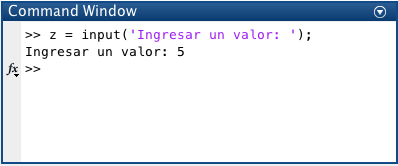
\includegraphics[scale=0.3]{images/pantalla1.png}
\end{center}
\end{column}
\begin{column}{0.3\textwidth}
\begin{center}
Workspace
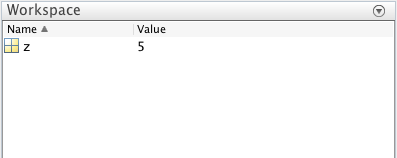
\includegraphics[scale=0.3]{images/pantalla2.png}
\end{center}
\end{column}
\end{columns}
\end{frame}

\begin{frame}{Entrada definida por el usuario}
Ej. Ejecutar las siguientes líneas. Obtener conclusiones.
\lstinputlisting[xleftmargin=.3\textwidth]{scripts/ej1.m}
\begin{columns}
\begin{column}{0.5\textwidth}
\begin{center}
Command windows
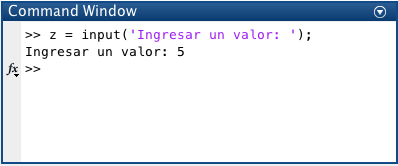
\includegraphics[scale=0.3]{images/pantalla1.png}
\end{center}
\end{column}
\begin{column}{0.3\textwidth}
\begin{center}
Workspace
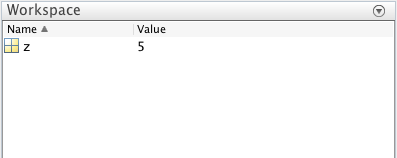
\includegraphics[scale=0.3]{images/pantalla2.png}
\end{center}
\end{column}
\end{columns}
\begin{block}{Tener en cuenta}
Puede ingresarse matrices, cadena de caracteres, entre otros
\end{block}
\end{frame}

\begin{frame}{Ejercicio práctico 10}
\begin{enumerate}
\item Cree un archivo .m para calcular el área de un triángulo. Permita al usuario ingresar los valores para la base y la altura.
\item Cree un archivo .m para encontrar el volumen de un cilíndro circular recto.
\item Cree un vector desde 1 hasta n, y permita al usuario ingresar el valor de n.
\item Cree un vector que comience en a, termine en b y tenga un espacio de c. Permita al usuario ingresar todos estos parámetros.
\end{enumerate}
\end{frame}

\begin{frame}{Opciones de salida}
\begin{exampleblock}{Comando}
Ver comando: \textbf{disp(x)}
\end{exampleblock}
\end{frame}

\begin{frame}{Opciones de salida}
\begin{exampleblock}{Comando}
Ver comando: \textbf{disp(x)}
\end{exampleblock}
\begin{center}
\textit{La función \textbf{disp} despliega los contenidos de una matriz sin imprimir el nombre de matriz.}
\end{center}
\end{frame}

\begin{frame}{Opciones de salida}
Ej. Ejecutar las siguientes líneas. Obtener conclusiones.
\lstinputlisting[xleftmargin=.3\textwidth]{scripts/ej2.m}
\end{frame}

\begin{frame}{Opciones de salida}
Ej. Ejecutar las siguientes líneas. Obtener conclusiones.
\lstinputlisting[xleftmargin=.1\textwidth]{scripts/ej3.m}
\begin{exampleblock}{Comando}
Ver comando: \textbf{num2str(x)}
\end{exampleblock}
\end{frame}

\begin{frame}{Salida formateada}
\begin{exampleblock}{Comando}
Ver comando: \textbf{fprintf(x)}
\end{exampleblock}
\begin{center}
\textit{Qué diferencia \textbf{fprintf()} de \textbf{disp()}?}
\end{center}
\end{frame}

\begin{frame}{Salida formateada}
\begin{exampleblock}{Comando}
Ver comando: \textbf{fprintf(x)}
\end{exampleblock}
\begin{center}
\textit{Qué diferencia \textbf{fprintf()} de \textbf{disp()}?}
\end{center}
\begin{columns}
\begin{column}{0.5\textwidth}
\begin{center}
La función \textbf{fprintf} además de desplegar los valores permite especificar el formato y saltos de línea
\end{center}
\end{column}
\begin{column}{0.5\textwidth}
\begin{center}

\includegraphics[scale=0.2]{images/img40.png}
\end{center}
\end{column}
\end{columns}
\end{frame}

\begin{frame}{Salida formateada}
Ej. Ejecutar las siguientes líneas. Obtener conclusiones.
\lstinputlisting[xleftmargin=.2\textwidth]{scripts/ej4.m}
\end{frame}

\begin{frame}{Salida formateada}
\textbf{Marcadores de posición:}
\begin{table}[]
\centering
\begin{tabular}{|c|c|}
\hline
Tipo de campo & Resultado                      \\ \hline
\%f           & Notación punto fijo o decimal  \\ \hline
\%e           & Notación exponencial           \\ \hline
\%g           & La que sea más corta \%f ó \%e \\ \hline
\%c           & Información carácter           \\ \hline
\%s           & Cadena de caracteres           \\ \hline
\end{tabular}
\end{table}
\end{frame}

\begin{frame}{Salida formateada}
Ej. Ejecutar las siguientes líneas. Obtener conclusiones.
\lstinputlisting[xleftmargin=.2\textwidth]{scripts/ej5.m}
\end{frame}

\begin{frame}{Salida formateada}
Ej. Ejecutar las siguientes líneas. Obtener conclusiones.
\lstinputlisting[xleftmargin=.2\textwidth]{scripts/ej5.m}
\begin{block}{Tener en cuenta}
Para indicar nueva línea utilizar el comando de formato: \textbf{\textbackslash n}
\end{block}
\end{frame}

\begin{frame}{Salida formateada}
\textbf{Comandos de formato:}
\begin{table}[]
\centering
\begin{tabular}{|c|c|}
\hline
Comando de formato & Acción resultante     \\ \hline
\textbackslash{}n  & Salto de línea        \\ \hline
\textbackslash{}r  & Regreso de carro      \\ \hline
\textbackslash{}t  & Tabulador             \\ \hline
\textbackslash{}b  & Retroceder un espacio \\ \hline
\end{tabular}
\end{table}
\end{frame}

\begin{frame}{Salida formateada}
Ej. Ejecutar las siguientes líneas. Obtener conclusiones.
\lstinputlisting[xleftmargin=.2\textwidth]{scripts/ej6.m}
\end{frame}

\begin{frame}{Salida formateada}
\begin{alertblock}{Importante}
Para incluir el signo porcentaje en un enunciado fprintf, se debe ingresar \%\% dos veces de lo contrario se interpretara \% como marcador de posición para datos
\end{alertblock}
\begin{center}

\includegraphics[scale=0.4]{images/img41.png}
\end{center}
\end{frame}

% %%%%%%%%%%%%%%%%%%%%%%%%%%%%%%%%%%%%%%%%%%%%%%%%%%%%%%%%%%%%%%%%%%%%%

% % Sección de consultas

% %%%%%%%%%%%%%%%%%%%%%%%%%%%%%%%%%%%%%%%%%%%%%%%%%%%%%%%%%%%%%%%%%%%%%

% \section{Consultas}
% \begin{frame}{Consultas}
% \begin{center}
% 
\includegraphics[scale=0.3]{images/consultas.png}
% \end{center}
% \end{frame}


% %%%%%%%%%%%%%%%%%%%%%%%%%%%%%%%%%%%%%%%%%%%%%%%%%%%%%%%%%%%%%%%%%%%%%

% % Sección de bibliografía

% %%%%%%%%%%%%%%%%%%%%%%%%%%%%%%%%%%%%%%%%%%%%%%%%%%%%%%%%%%%%%%%%%%%%%

% \section{Bibliografia}

% \begin{frame}{Bibliografía}
% \begin{columns}
% \begin{column}{0.5\textwidth}
% \begin{center}
% 
\includegraphics[scale=0.4]{images/biblio1.png}
% \end{center}
% \end{column}
% \begin{column}{0.5\textwidth}
% \begin{center}
% 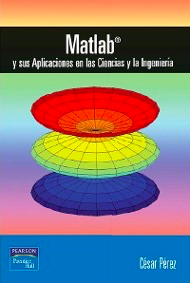
\includegraphics[scale=0.5]{images/biblio2.png}
% \end{center}
% \end{column}
% \end{columns}
% \end{frame}

\end{document}
